%% -*- coding:utf-8 -*-
\begin{figure}
\centering

\ifpdf
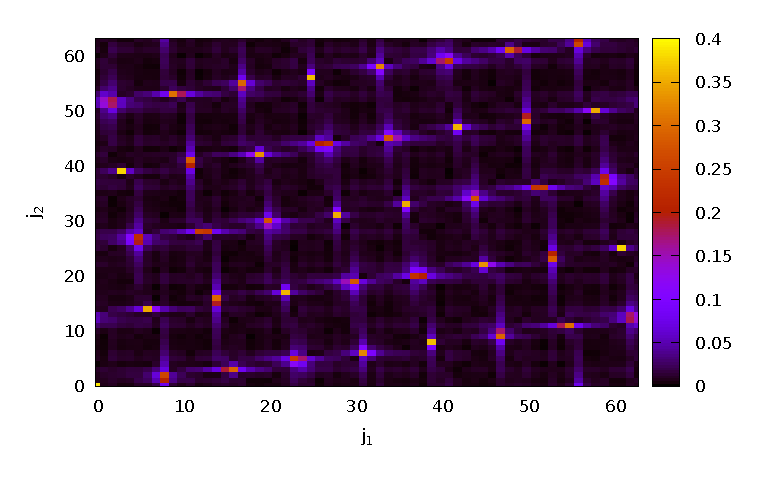
\includegraphics[angle=0]
{./part4/quantcomp/picellipticdiscretlog2.pdf}
\else
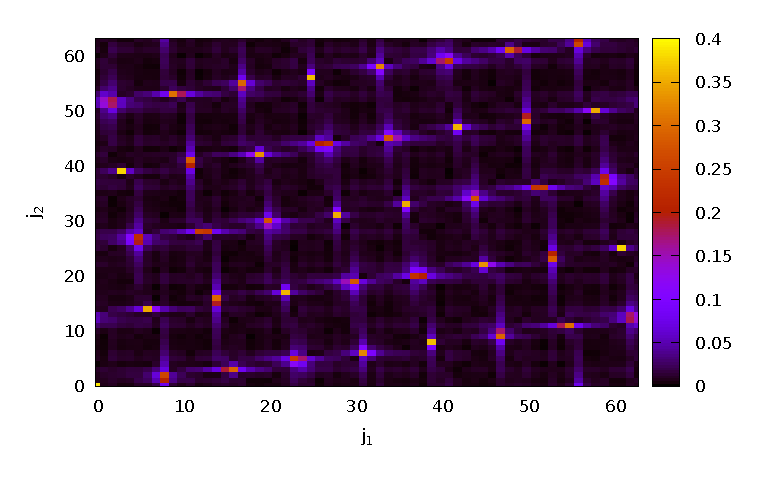
\includegraphics[angle=0]
{./part4/quantcomp/picellipticdiscretlog2.eps}
\fi

%\input ./part4/quantcomp/picdiscretlog2.tex

\caption{Фурье образ отсчетов функции 
$f'(x_1, x_2)$
Число отсчетов $M=64$. Три левых нижних максимума имеют координаты $\approx (8,2), (15,3), (24,5)$, что дает следующие оценки для $x$: $x \approx 4, 5, 4.8$,
что находится близко к реальному значению $x = 5$
} 
\label{fig:part4:quantcomp:dle2}
\end{figure}
